\chapter{Even infinity admits a hierarchy we must confront: The Real Numbers}

\begin{figure}[ht]       
\centerline{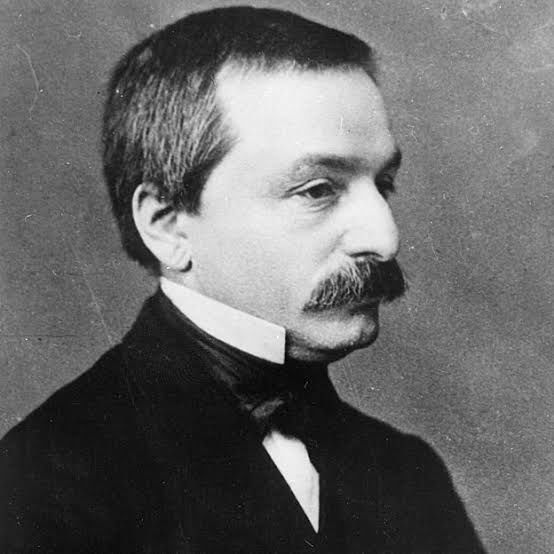
\includegraphics[width=1.0in]{images/kronecker.jpeg}}
\caption*{\small ``God created the integers; all else is the work of man'' -- \href{https://en.wikipedia.org/wiki/Leopold\_Kronecker}{Leopold Kronecker}}
\end{figure}

\begin{figure}[ht]       
\centerline{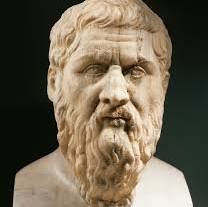
\includegraphics[width=1.0in]{images/plato2.jpeg}}
\caption*{\small ``He is unworthy of the name of man who is ignorant of the fact that the diagonal of a square is incommensurable with its side'' -- \href{https://en.wikipedia.org/wiki/Plato}{Plato}}
\end{figure}
%\epigraph{``God created the integers; all else is the work of man.''}{\textit{Leopold Kronecker (1886)}}



The real numbers are the backbone of modern mathematics. They unify discrete and continuous quantities, allow us to measure lengths, areas, speeds, and forces, and they form the natural domain for calculus, physics, probability, and geometry. Yet the construction of the real numbers is not obvious, and their necessity arises from deep conceptual difficulties that puzzled mathematicians for millennia.

In this chapter we try to build a conceptual and computational foundation for understanding the real numbers, their structure, and the functions defined on them.

\bigskip

%%%%%%%%%%%%%%%%%%%%%%%%%%%%%%%%%%%%%%%%%%%%%%%%%%%%%%%%%%%%%%
\section{Why Do We Need Real Numbers?}

As we saw earlier in these notes, mathematics begins with the natural numbers $\mathbb{N}$,  which suffice for counting and simple arithmetic. But subtraction motivates the integers $\mathbb{Z}$, division motivates the rationals $\mathbb{Q}$, and geometry quickly reveals that even rational numbers are insufficient.  


%\subsection{Why Rational Numbers Are Not Enough}
%
%Examples that push us out of $\mathbb{Q}$:
%
%\begin{itemize}
%\item $\sqrt{2}, \sqrt{3}$ from geometry.
%\item $\pi$ from circle circumference and area.
%\item $e$ from continuous growth.
%\item Infinite decimals such as $0.1010010001\ldots$.
%\end{itemize}
%
%All of these lie outside $\mathbb{Q}$.

\subsection{Incompleteness of the Rationals and the irrational persecution of \href{https://en.wikipedia.org/wiki/Hippasus}{Hippasus}}

In Theorem \ref{thm:sqrt2} we discussed a  classical proof  that shows that $\sqrt{2}\notin \mathbb{Q}$. This was shocking in antiquity and led to the development of more sophisticated number systems. Thus geometry forces us beyond the rationals.

\begin{quote}
``He is unworthy of the name of man who is ignorant of the fact that the diagonal of a square is incommensurable with its side''\quad -- (Plato)
\end{quote}

\href{https://en.wikipedia.org/wiki/Hippasus}{Hippasus} is often credited with the discovery of irrational numbers. According to common folklore the Pythagoreans was rather upset with this discovery, and Hippasus is supposed to have drowned at sea, apparently as a punishment from the gods for divulging this troublesome fact.

There are more reason as to why rational are incomplete. Although $\mathbb{Q}$ is dense on the line, it contains ``holes''. A sequence of rational numbers may converge to a limit that is not rational.

Consider, for example,
\[
y_n = \sum_{k=1}^n 10^{-k!}
\]
Each $y_n$ is rational, but the limit is the Liouville constant, which is not rational.

\begin{theorem}
The \href{https://en.wikipedia.org/wiki/Liouville\_number}{Liouville constant}
\[
L = \sum_{k=1}^{\infty} \frac{1}{10^{k!}}
= \frac{1}{10}+\frac{1}{10^{2}}+\frac{1}{10^{6}}+\frac{1}{10^{24}}+\cdots
\]
is irrational.
\end{theorem}

\begin{proof}
We will use the fact that a decimal number is rational if and only if its decimal expansion is
\emph{eventually periodic}; that is, after some point its digits repeat with a
fixed period. We will prove this in a exercise problem at the end of this chapter.

Let us analyse the decimal expansion of $L$.  The term $\tfrac{1}{10^{k!}}$
contributes a single `1' in the $k!$-th decimal place and zeros elsewhere.
Thus $L$ has a `1' in the decimal positions
\[
1!, \; 2!,\; 3!,\; 4!,\; \dots
\]
and all other digits are $0$.  Therefore the distances between successive
positions of `1' are
\[
\begin{array}{c}
2! -1! = 1  \\
3! - 2! =4 \\
4! - 3! =18 \\
5! -4! =96 \\
\end{array}
\]
and in general

\[
(k+1)! - k! = k!\cdot k
\]


These gaps grow without bound as $k\to\infty$.

Now suppose, for the sake of contradiction, that $L$ is rational.  Then its
decimal expansion would be eventually periodic: there exist integers $N\ge 1$
and $p\ge 1$ such that all digits from position $N$ onward repeat with period
$p$.  In particular, after position $N$, if a digit `1' occurs once, then the
same digit `1' must occur again exactly $p$ places later, and then again $p$
places after that, and so on.  Thus the distances between successive `1's
beyond $N$ must all be \emph{exactly} $p$.

However, choose $k$ large enough that $k!\cdot k > p$ and also $k! > N$.
Then between the `1' at position $k!$ and the next `1' at position $(k+1)!$
there are
\[
(k+1)! - k! = k!\cdot k
\]
zeros --- a gap strictly greater than $p$.  This contradicts the assumption
that the decimal expansion is eventually periodic with period $p$.

Hence no such period $p$ can exist, and the decimal expansion of $L$ is not
eventually periodic.  Therefore $L$ is irrational.
\end{proof}


Hence, rhe rational numbers are not complete. Limits of rational sequences need not be rational. To properly define limits, infinite series, areas, lengths, and solutions of differential equations, we need a larger number system.

\subsection{Zeno's paradox and infinite processes: Achilles and the Tortoise}

\href{https://en.wikipedia.org/wiki/Zeno\_of\_Elea}{Zeno of Elea (5th century BCE)} presented several paradoxes to argue that
motion is impossible.  His most famous example is the paradox of
\emph{Achilles and the Tortoise}, which troubled mathematicians and
philosophers for centuries.  We now explain the paradox in detail and
show how it naturally leads to the concept of limits and infinite series.

\subsubsection*{The Setup}

Suppose Achilles, the fastest of the Greek heroes, runs ten times faster
than a tortoise.  The tortoise is given a head start of $D$ metres.
Common sense says Achilles will quickly overtake the tortoise.  Zeno's
reasoning, however, appeared to show otherwise.

\subsubsection*{Zeno's Argument}

Zeno argued as follows:
\begin{enumerate}
    \item Achilles first runs to the tortoise's starting point (distance $D$).
    \item During that time, the tortoise moves ahead a little.
    \item Achilles then runs to this new position.
    \item Again the tortoise moves slightly ahead.
    \item This continues forever, \emph{ad infinitum}.
\end{enumerate}

Thus Achilles must complete \emph{infinitely many tasks}:
first reach $D$, then $D(1+r)$, then $D(1+r+r^2)$, and so on, where
$r$ is the ratio of the tortoise's speed to Achilles' speed.
Zeno concluded that Achilles can never overtake the tortoise.

\subsubsection*{Mathematical Formulation}

Let $v_A$ be Achilles' speed and $v_T$ be the tortoise's speed, with
$v_A > v_T$.  Let the tortoise's head start be $D$.

The time Achilles takes to reach the tortoise's initial position is
\[
t_1 = \frac{D}{v_A}.
\]
During this time the tortoise moves
\[
D_1 = v_T t_1 = D\cdot \frac{v_T}{v_A}.
\]

Next, Achilles takes
\[
t_2 = \frac{D_1}{v_A} = \frac{D}{v_A}\left(\frac{v_T}{v_A}\right)
\]
to reach that point; during this period the tortoise moves
\[
D_2 = D \left(\frac{v_T}{v_A}\right)^2.
\]

Continuing, we obtain an infinite sequence of positive times
\[
t_1, \; t_2, \; t_3,\; \dots
\]
with
\[
t_n = \frac{D}{v_A}\left(\frac{v_T}{v_A}\right)^{n-1}.
\]

Thus the total time required for Achilles to reach all points previously
occupied by the tortoise is
\[
T = t_1 + t_2 + t_3 + \cdots
 = \frac{D}{v_A}
   \left(1 + r + r^2 + r^3 + \cdots\right),
\]
where
\[
r = \frac{v_T}{v_A} \quad \text{and} \quad 0 < r < 1.
\]

\subsubsection*{Resolution via convergent geometric series}

We will show in Section \ref{sec:apgp} that the  infinite geometric series with $0 < r < 1$ satisfies
\[
1 + r + r^2 + r^3 + \cdots = \frac{1}{1-r}.
\]

Hence
\[
T
 = \frac{D}{v_A}\cdot \frac{1}{1-r}
 = \frac{D}{v_A - v_T}.
\]

That is, the infinite sum actually converges to a finite quantity, a rational number if $r$ is rational. This is the standard ``relative speed'' formula for the time taken for a
faster runner to catch a slower one.  The total time $T$ is finite.

\emph{Achilles does indeed overtake the tortoise.}

\subsubsection*{What Zeno misunderstood}

Zeno implicitly assumed that a process involving infinitely many steps
must take an infinite amount of time.  Modern mathematics shows that
an infinite series of positive quantities may converge to a finite sum.
Here the quantities $t_n$ become smaller so rapidly that their infinite
sum remains finite.

This is only made rigorous in the \emph{real numbers}, which allow us to
define limits and convergent series.  In this sense, Zeno's paradox
hints at the need for a complete number system.


%Bertrand Russell famously observed:
%\begin{quote}
%``Zeno's arguments were designed to bring out contradictions implicit
%in the ordinary ideas of space and time.''
%\end{quote}

\begin{figure}[ht]       
\centerline{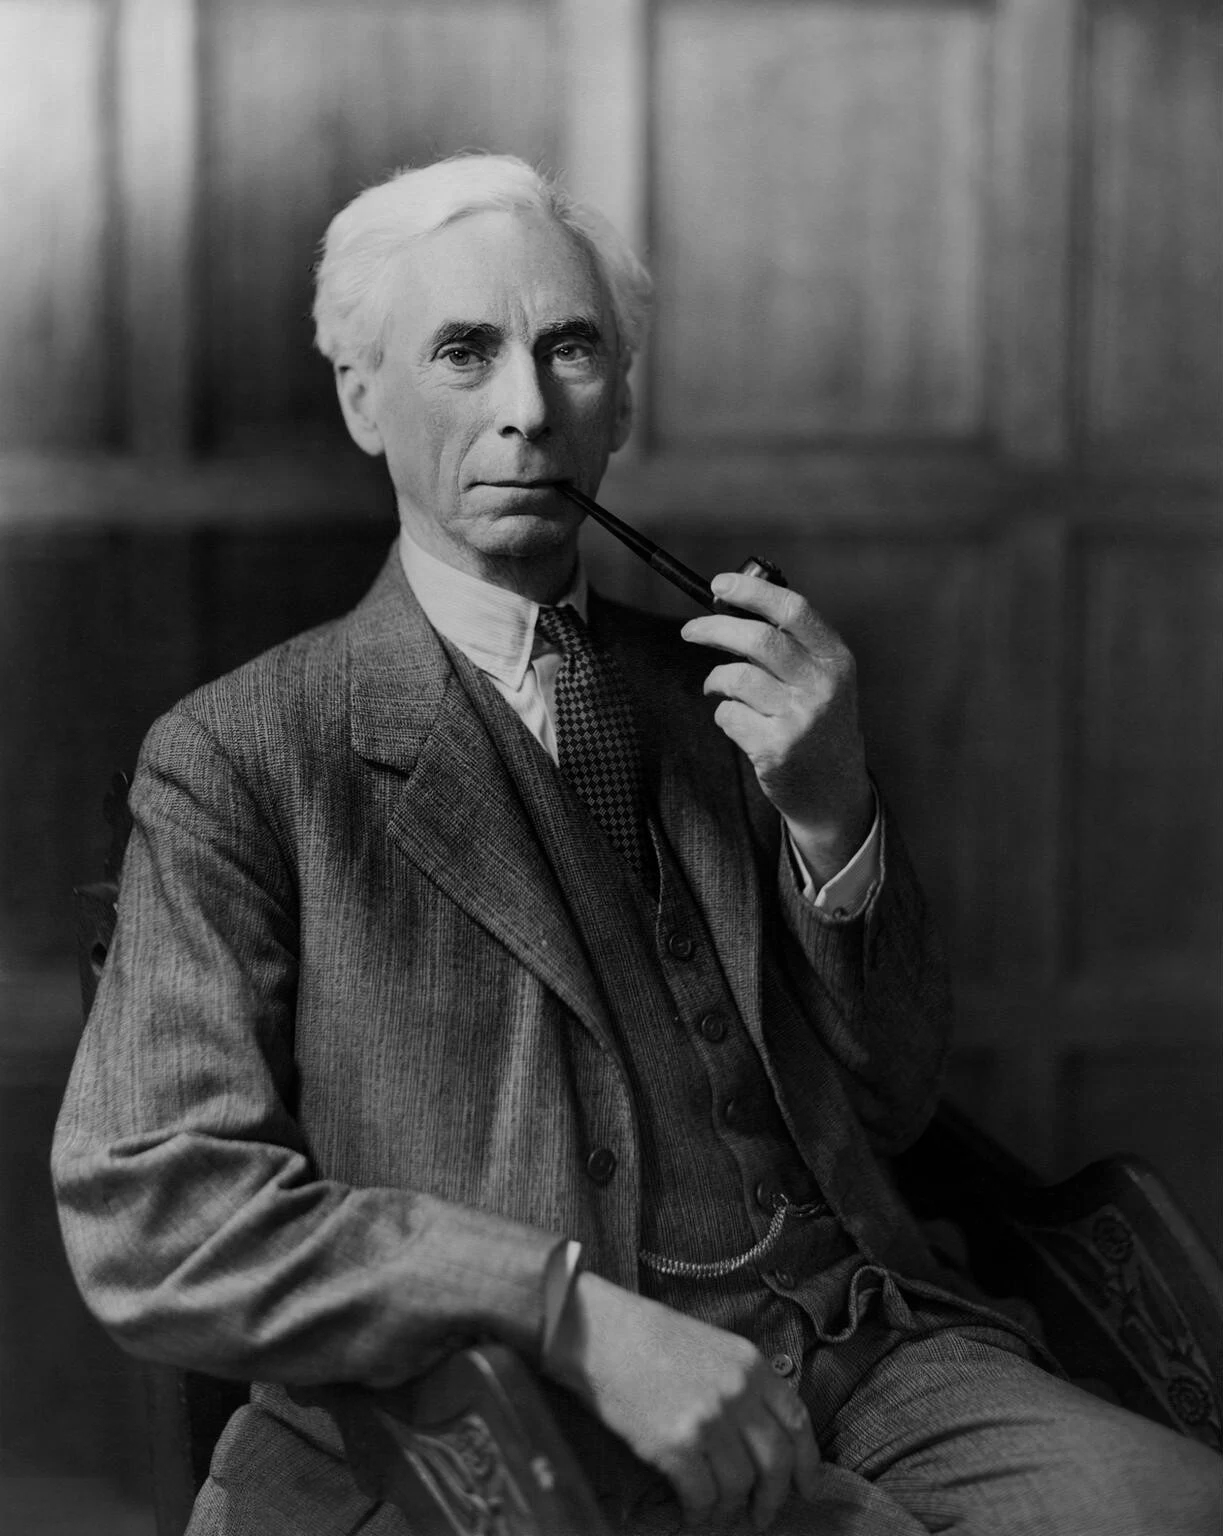
\includegraphics[width=1.0in]{images/russel2.jpg}}
\caption*{\small ``The paradoxes of Zeno the Eleatic and the difficulties in the analysis of space, 
of time, and of motion, are all completely explained by means of the modern 
theory of continuity. This is because a non-contradictory theory has been 
found, according to which the continuum is composed of an infinity of distinct 
elements; and this formerly appeared impossible'' --  \href{https://en.wikipedia.org/wiki/Bertrand_Russell}{Bertrand Russell}}
\end{figure}
\begin{figure}[ht]       
\centerline{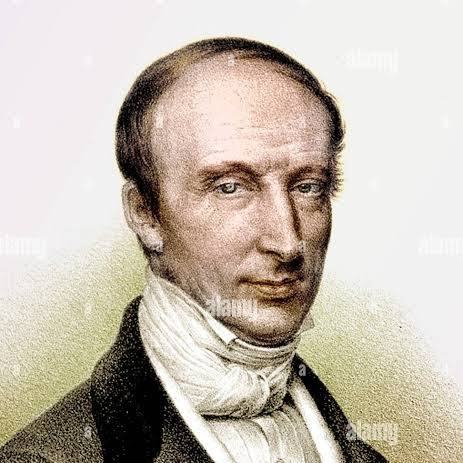
\includegraphics[width=1.0in]{images/cauchy.jpg}}
\caption*{\small ``It is by the idea of limit alone that the calculus becomes a rigorous science.'' --  \href{https://en.wikipedia.org/wiki/Augustin-Louis_Cauchy}{A.–L. Cauchy}, Cours d’Analyse (1821)}
\end{figure}
\begin{figure}[ht]       
\centerline{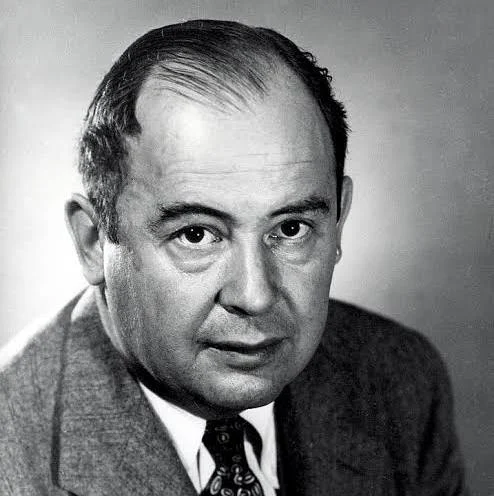
\includegraphics[width=1.0in]{images/vonneumann.png}}
\caption*{\small ``The calculus was the first achievement of modern mathematics and it is difficult to overestimate its importance. I think it defines more unequivocally than anything else the inception of modern mathematics; and the system of mathematical analysis, which is its logical development, still constitutes the greatest technical advance in exact thinking.'' --  \href{https://en.wikipedia.org/wiki/John_von_Neumann}{John von Neumann}}
\end{figure}


Understanding the resolution of Zeno's paradox requires understanding limits, convergence, and the structure of the real numbers. 
The resolution uses \emph{infinite series} and the idea of a \emph{limit}. These require a complete number system --- the real numbers. A follow up course on \emph{Calculus} is strongly recommended.

\section{The Real Line as a Continuum}

One way to view the real line is as the set of all (possibly infinite, non-repeating) decimals. Another is to view the real line as the completion of the rationals under limits of Cauchy sequences.

\begin{definition}[Cauchy Sequence]
A sequence $(x_n)$ of real or rational numbers is called a \emph{Cauchy
sequence} if for every $\varepsilon>0$ there exists $N\in\mathbb{N}$
such that for all $m,n\ge N$,
\[
|x_m - x_n| < \varepsilon.
\]
\end{definition}

In other words, the terms of the sequence eventually become arbitrarily
close to one another.  It turns out that every Cauchy sequence converges in $\mathbb{R}$,
but not necessarily in $\mathbb{Q}$, which shows that the rationals are
not complete.


\subsection{Cantor: The Reals are uncountable}

\begin{figure}[ht]       
\centerline{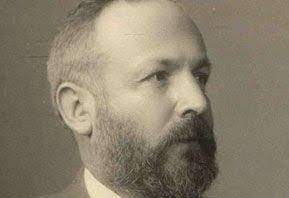
\includegraphics[width=1.0in]{images/cantor2.jpeg}}
\caption*{\small ``I see it, but I don't believe it!'' -- \href{https://en.wikipedia.org/wiki/Georg_Cantor}{Georg Cantor}}
\end{figure}

In 1874, Cantor used his celebrated \emph{diagonal argument} to prove that no list can contain all real numbers in $(0,1)$.

\begin{theorem}[Cantor's Diagonal Argument]
The interval $(0,1)$ is uncountable.  In particular, there is no bijection
between the natural numbers $\mathbb{N}$ and the real numbers in $(0,1)$.
\end{theorem}

\begin{proof}
Suppose, for the sake of contradiction, that $(0,1)$ is countable.
Then every real number in $(0,1)$ has a decimal expansion of the form
\[
0.a_1 a_2 a_3 \dots,
\]
and our assumption implies that it is possible to list \emph{all} such
numbers in a single infinite sequence.  Thus suppose we have an
enumeration
\[
x_1, x_2, x_3, \ldots
\]
of all real numbers in $(0,1)$, where each $x_n$ is written in decimal
form as
\[
\begin{array}{ccc}
x_1 & = & 0.a_{11} a_{12} a_{13} a_{14} \dots \\
x_2 & = & 0.a_{21} a_{22} a_{23} a_{24} \dots \\
       & \vdots & \\
x_n & = & 0.a_{n1} a_{n2} a_{n3} a_{n4} \dots \\
  & \vdots & \\
\end{array}
\]
Here $a_{nk} \in \{0,1,2,\dots,9\}$ is the $k$-th digit of the $n$-th
number in the list.

\medskip
\noindent\emph{Important convention.}  
To avoid the ambiguity of decimal expansions such as
$0.2499999\ldots = 0.25$, we assume that no number in the list ends in
an infinite tail of $9$'s.  Every real number in $(0,1)$ has at least one
representation without trailing $9$'s, so this assumption does not omit
any real number.

\medskip
Now we construct a new number $y$ whose decimal digits differ from
the diagonal digits of the list.  Define
$y = 0.b_1 b_2 b_3 \dots$ by
\[
b_k =
\begin{cases}
5, &\text{if } a_{kk} \neq 5,\\[4pt]
4, &\text{if } a_{kk} = 5.
\end{cases}
\]
In other words, $b_k$ is chosen so that it \emph{differs} from $a_{kk}$.
This is always possible because there are ten possible digits, and we
deliberately avoid choosing the digit $9$, so $y$ will not end in an
infinite string of $9$'s.

\medskip
Consider any index $n\in\mathbb{N}$.  We compare $y$ with the $n$-th
number $x_n$ in the list.  The $n$-th digit of $x_n$ is $a_{nn}$, while
the $n$-th digit of $y$ is $b_n$, which was chosen to be \emph{different}
from $a_{nn}$.  Therefore,
\[
y \neq x_n.
\]

Since this argument holds for every $n$, we conclude that the constructed
number $y$ is different from $x_n$ for all $n\in\mathbb{N}$.  But this
contradicts our assumption that $(0,1)$ was completely enumerated by the
sequence $x_1, x_2, x_3, \dots$.

\medskip
Thus our original assumption was false.  No such complete enumeration
exists, and therefore $(0,1)$ is uncountable.
\end{proof}

\begin{figure}[ht]       
\centerline{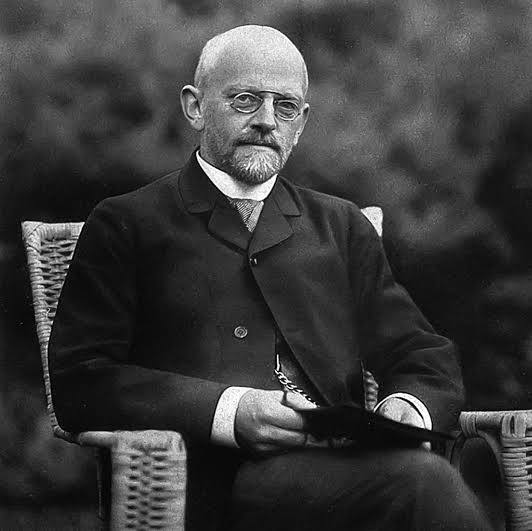
\includegraphics[width=1.0in]{images/hilbert.jpeg}}
\caption*{\small ``No one shall expel us from the paradise that Cantor has created.'' --  \href{https://en.wikipedia.org/wiki/David_Hilbert}{David Hilbert}}
\end{figure}

The result was revolutionary and laid the foundations of modern set theory. Quite amazingly, \emph{diagonalization} as a  proof technique has also turned out to be foundational in logic and computer science.

%%%%%%%%%%%%%%%%%%%%%%%%%%%%%%%%%%%%%%%%%%%%%%%%%%%%%%%%%%%%%%
\section{Algebraic and Transcendental Numbers}
\label{sec:algebraicnumbers}
The irrationals split into two classes.

A real number $x$ is \emph{algebraic} if it is a root of (a solution of) an equation like
\[
a_n x^n + a_{n-1}x^{n-1} + \cdots + a_1 x + a_0 = 0
\]
with rational coefficients $a_0, a_1,\dots,a_n$. Expressions such as the left hand side of the above equation are called \emph{polynomials} and the solutions are called its \emph{roots}.

Some examples are
\[
\sqrt{2},\qquad \sqrt[3]{5},\qquad \frac{1+\sqrt{5}}{2}
\]

If a number is not algebraic, it is \emph{transcendental}.  
Some famous examples are $e$ and $\pi$ which will soon discuss.


\href{https://en.wikipedia.org/wiki/Liouville\_number}{Liouville (1844)} constructed numbers that are ``too well approximated'' by rationals:
\[
L = \sum_{k=1}^\infty 10^{-k!}
\]
Liouville proved that $L$ is transcendental.

\begin{quote}
``Transcendental numbers are not rare; they are, in fact, the rule.''  
\textit{--- \href{https://en.wikipedia.org/wiki/Kurt_Mahler}{Kurt Mahler}}
\end{quote}

%%%%%%%%%%%%%%%%%%%%%%%%%%%%%%%%%%%%%%%%%%%%%%%%%%%%%%%%%%%%%%
\subsection{How fast do our money grow? Simple and compound interests}

When we invest  in a financial instrument our money earns \emph{interest} and grows.

\emph{Simple interest}
assumes that interest is calculated only on the original principal, and
that previously earned interest does not itself earn further interest.

Let
\[
P = \text{principal (initial amount)}, \qquad
r = \text{annual interest rate}, \qquad
t = \text{time in years}.
\]
Under simple interest, the total amount after $t$ years is
\[
A(t) = P(1 + rt).
\]

This is a linear function of $t$.  The amount increases at a constant
rate $Pr$ per year, so the graph of $A(t)$ against $t$ is a straight line.

\begin{example}
Suppose you invest
\[
P = \mbox{\rupee}10{,}000 
\]
at an annual simple interest rate of $r = 0.08$ (i.e.\ 8\% per year). Then

\vspace{0.25in}
\begin{tabular}{ll}
\hline
After 1 year: &  $A(1) = 10000(1 + 0.08) = 10800$ \\
After 3 years: &  $A(3) = 10000(1 + 0.08\times 3) = 10000(1 + 0.24) = 12400$ \\
After 10 years: & $A(10) = 10000(1 + 0.08\times 10)  = 10000(1 + 0.80) = 18000$ \\
\hline
\end{tabular}
\vspace{0.25in}

In each year, the amount increases by the same amount:
\[
Pr = 10000\times 0.08 = \mbox{\rupee} 800 
\]
\end{example}


Under \emph{compound interest}, interest is added periodically and in each period
the previously earned interest itself earns further interest.  If $P$ is
the principal, $r$ is the annual interest rate, and interest is compounded
once per year, then the amount after $t$ years is
\[
A_c(t) = P(1+r)^{t}.
\]

\begin{example}
For the same values as in the simple–interest example,
\[
P = 10{,}000,\qquad r = 0.08,
\]
we obtain
\[
A_c(t)=10000(1.08)^t
\]
Thus,

\vspace{0.25in}
\begin{tabular}{ll}
\hline
After 1 year: &  $A(1) = 10000(1.08) = 10800$ \\
After 3 years: &  $A(3) = 10000(1.08)^3 = 12597.12 $ \\
After 10 years: & $A(10) = 10000(1.08)^10  = 21589.25$ \\
\hline
\end{tabular}
\vspace{0.25in}

\end{example}

While simple interest grows linearly, compound interest grows
exponentially.  Over long durations the difference becomes significant, 
and compounded growth eventually ``pulls away'' from linear
growth.

\begin{figure}[h]
\centering
\resizebox{0.7\textwidth}{!}{%
\begin{tikzpicture}[scale=0.85]

% ----- Axes -----
\draw[->] (0,0) -- (21,0) node[right] {Time $t$ (years)};
\draw[->] (0,0) -- (0,8) node[above] {Amount (rupees)};

% y-axis ticks (scaled: +5000 rupees = +1 unit)
\foreach \y/\lab in {0/10, 1/15, 2/20, 3/25, 4/30, 5/35, 6/40, 7/45, 8/50} {
    \draw (-0.15,\y) -- (0.15,\y);
    \node[left] at (-0.25,\y) {\lab,000};
}

% x-axis ticks
\foreach \x in {0,5,10,15,20} {
    \draw (\x,0) -- (\x,-0.15);
    \node[below] at (\x,-0.2) {\x};
}

% ----- Simple interest: y=0.16 t -----
\draw[thick] (0,0) -- (20,3.2);
\foreach \t/\y in {0/0, 5/0.8, 10/1.6, 15/2.4, 20/3.2} {
    \fill (\t,\y) circle (2pt);
}

% ----- Compound interest: annual -----
% Precomputed values:
% t=0: 10000       -> y=0
% t=5: 14693.28    -> y=0.938656
% t=10: 21589.25   -> y=2.31785
% t=15: 31721.64   -> y=4.34433
% t=20: 46517.34   -> y=7.30347

\draw[thick, dashed]
    plot[smooth] coordinates {
        (0,0)
        (5,0.938656)
        (10,2.31785)
        (15,4.34433)
        (20,7.30347)
    };

\foreach \t/\y in {0/0, 5/0.938656, 10/2.31785, 15/4.34433, 20/7.30347} {
    \fill (\t,\y) rectangle ++(0.12,0.12);
}

% ----- Legend -----
\begin{scope}[shift={(12,7.2)}]
    \draw[thick] (0,0) -- (1,0);
    \node[right] at (1.2,0) {Simple interest};

    \draw[thick, dashed] (0,-0.7) -- (1,-0.7);
    \node[right] at (1.2,-0.7) {Compound interest};
\end{scope}

\end{tikzpicture}%
}
\caption{Simple vs annually compounded growth at $8\%$ for $P=10{,}000$ over 20 years.
Vertical scale: $y=(A(t)-10000)/5000$.}
\end{figure}

As $n$ increases, this expression approaches the continuously compounded
growth
\[
A(t) = Pe^{rt},
\]
revealing the natural appearance of the constant $e$.  Thus the transition
from simple to compound interest provides a natural pathway from linear
to exponential growth.

\subsection{From compound interest to the number \texorpdfstring{$e$}{e}}

Compound interest provides a natural setting in which the exponential
number $e$ appears.  Suppose a principal amount $P$ is invested at an
annual interest rate $r$, but interest is now credited not once a year,
but $n$ times per year.  In each compounding period the interest rate is
$r/n$, so the amount after one year becomes
\[
A_n(1) = P\left(1 + \frac{r}{n}\right)^{n}.
\]

For example:
\begin{itemize}
    \item with $n=1$ (annual compounding), we obtain $P(1+r)$,
    \item with $n=4$ (quarterly compounding), we obtain
    $P\left(1+\frac{r}{4}\right)^4$,
    \item with $n=12$ (monthly compounding), we obtain
    $P\left(1+\frac{r}{12}\right)^{12}$,
    \item with $n=365$ (daily compounding), we obtain
    $P\left(1+\frac{r}{365}\right)^{365}$.
\end{itemize}

As $n$ increases, interest is credited more and more frequently, and the
amount grows slightly larger.  A natural mathematical question is:
\[
\textit{What happens as } n \to \infty?
\]

\medskip
\noindent
To study this limit, let us first focus on the core expression
\[
\left(1 + \frac{1}{n}\right)^{n}.
\]
One can check numerically that
\[
\left(1+\frac{1}{n}\right)^n
=
2.0000,\; 2.2500,\; 2.3707,\; 2.3979,\; 2.7048,\;\dots
\]
for $n=1,2,3,4,10,\dots$, and that the sequence increases and approaches
a limiting value.  This limit is denoted by the symbol $e$\footnote{Estimating its value will require some advanced techniques which an interested reader may look up.}.
\[
e = \lim_{n\to\infty}\left(1+\frac{1}{n}\right)^{n} \approx  2.71828
\]

The limit can also be written as an infinite sum. The full Binomial expansion becomes
\[
\left(1+\frac{1}{n}\right)^{n}
=
1
+ 1
+ \frac{1}{2}\left(1-\frac{1}{n}\right)
+ \frac{1}{6}\left(1-\frac{1}{n}\right)\left(1-\frac{2}{n}\right)
+ \cdots.
\]

As $n\to\infty$, $\frac{1}{n}\to 0$, Hence,
\[
e = 1 + 1 + \frac{1}{2!} +  \frac{1}{3!} +  \frac{1}{4!} + \cdots
\]

\vspace{0.25in}
Thus, continuous compounding at rate $r$ leads to the amount
\[
A(1)=Pe^{\,r}
\]

\noindent
In general, after $t$ years the continuously compounded amount becomes\footnote{\href{https://en.wikipedia.org/wiki/Jacob_Bernoulli}{Jacob Bernoulli} discovered this limit while studying compound interest in 1683. \href{https://en.wikipedia.org/wiki/Leonhard_Euler}{Leonhard Euler} later linked it to calculus and defined it analytically.}
\[
A(t)=Pe^{\,rt}.
\]
This is the fundamental exponential-growth formula.  The appearance of
$e$ is therefore not mysterious: it arises naturally as the limiting
value of compound interest when interest is credited infinitely often.

\begin{quote}
\emph{``The number $e$ is the unique real number for which continuous
growth at rate 1 yields a unit increase in one time unit.''}
\end{quote}

This interpretation makes $e$ one of the most important constants in
mathematics, appearing in finance, probability theory, calculus,
differential equations, and many dynamical processes in the natural and
social sciences.

%%%%%%%%%%%%%%%%%%%%%%%%%%%%%%%%%%%%%%%%%%%%%%%%%%%%%%%%%%%%%%
\subsection{The Number $\pi$ from Geometry}

All circles are similar: any circle can be obtained from any other by a
uniform scaling.  Under scaling by a factor $k>0$, every length is multiplied
by $k$.  Hence circumference and diameter scale by the same factor, so their
ratio is unchanged.

\begin{figure}[h]
\centering
\begin{tikzpicture}[scale=1]

% Small circle
\draw[thick] (-3,0) circle (1.2);
\fill (-3,0) circle (1pt);
\node at (-3,-1.7) {$\text{Circle of radius } r$};

% Radius arrow small
\draw[->] (-3,0) -- (-1.8,0) node[midway, above] {$r$};

% Diameter arrow small
\draw[<->] (-4.2,0) -- (-1.8,0) node[midway, below] {$D=2r$};

% label circumference
\node at (-3,1.55) {$C$};

% Big circle (scaled)
\draw[thick] (3,0) circle (2.2);
\fill (3,0) circle (1pt);
\node at (3,-2.7) {$\text{Circle of radius } kr$};

% Radius arrow big
\draw[->] (3,0) -- (5.2,0) node[midway, above] {$kr$};

% Diameter arrow big
\draw[<->] (0.8,0) -- (5.2,0) node[midway, below] {$D'=2kr=kD$};

% label circumference
\node at (3,2.55) {$C'$};

% Scaling arrow between circles
\draw[->, thick] (-0.4,1.8) -- (0.4,1.8);
\node at (0,2.1) {scale by $k$};

% Text below to emphasize ratio
\node[align=center] at (0,-4.0)
{$C' = kC,\quad D' = kD\quad\Rightarrow\quad \dfrac{C'}{D'}=\dfrac{C}{D}.$};

\end{tikzpicture}
\caption{Scaling a circle by factor $k$ multiplies both circumference and
diameter by $k$, so the ratio $C/D$ is the same for all circles.}
\end{figure}
\begin{definition}
For every circle,
\[
\pi = \frac{C}{D} = \frac{C}{2r}.
\]
\end{definition}

For a disk of radius $r$, the area is given as
\[
A(r) = \pi r^2.
\]

Thus $\pi = A(1)$: the area of the unit disk.

\subsubsection{Approximations of $\pi$}

\href{https://en.wikipedia.org/wiki/Archimedes}{Archimedes} approximated $\pi$ using inscribed and circumscribed $n$-gons. Using a $96$-gon, he showed
\[
3\frac{10}{71} < \pi < 3\frac{1}{7}.
\]

The \href{https://en.wikipedia.org/wiki/Leibniz_formula_for_\%CF\%80}{Leibniz formula for $\pi$} obtained using a geometric series approximation and integration is given as
\[
\frac{\pi}{4} = 1 - \frac13 + \frac15 - \frac17 + \cdots
\]
This series converges slowly but gives an exact expression.  This series is also sometimes called the Madhava-Leibniz series as it was first discovered by \href{https://en.wikipedia.org/wiki/Madhava_of_Sangamagrama}{Madhava of Sangamagrama}\footnote{See \href{https://en.wikipedia.org/wiki/Approximations_of_\%CF\%80}{https://en.wikipedia.org/wiki/Approximations\_of\_$\pi$} for a history of various approximations of $\pi$.}. It can be shown that $\pi$ is a transcendental number.


\section*{Problems}

\begin{enumerate}

\item (\textbf{Incompleteness of the rationals})
Give an example of a Cauchy sequence of rational numbers that does \emph{not} converge
to any rational number. Explain why this demonstrates a “gap’’ in $\mathbb{Q}$.

\item (\textbf{Achilles and the Tortoise})
In the Achilles–Tortoise setup where Achilles runs at twice the speed of the tortoise,
write the explicit geometric series representing Achilles’ motion.  
Compute its sum and argue why the paradox dissolves once infinite sums are allowed.

\item (\textbf{Density})
Prove that between any two irrational numbers there exists a rational number.
(Hint: scale and shift.)

\item (\textbf{Decimal expansions})
Give an example of a non-terminating repeating decimal and a non-repeating decimal.
Classify each as rational or irrational and justify your answer.

\item (\textbf{Cantor’s diagonal argument})
Explain why the diagonal method does not contradict the fact that decimal
representations have non-uniqueness (e.g.\ $0.4999\ldots = 0.5$).
Why does the argument still go through?

\item (\textbf{Countability vs uncountability})
Show that the set of all infinite binary sequences is uncountable
by giving a diagonal proof analogous to Cantor’s proof for $(0,1)$.

\item (\textbf{Algebraic vs transcendental})
Prove that the number
\[
L = \sum_{k=1}^\infty 10^{-k!}
\]
is irrational.  
(Hint: compare $L$ with rational numbers truncated after $n!$ decimal places.)

\item (\textbf{From compound interest to $e$})
Compute $\left(1+\frac{1}{n}\right)^{n}$ for $n=1,2,5,10,100,1000$.
Does the sequence appear to converge?
How does this motivate the definition of $e$?

\item (\textbf{$e$ as a limit})
Show that the sequence
\[
a_n = \left(1+\frac{1}{n}\right)^{n+1}
\]
is bounded above by $e$.  
(Hint: use monotonicity and the binomial expansion.)

\item (\textbf{Archimedes' method})
Using a circumscribed $n$-gon around a unit circle, derive an upper bound on $\pi$.
Compute the bound explicitly for $n=6$ and $n=12$.

\item (\textbf{Transcendentals exist “in abundance’’})
Show that the set of algebraic numbers is countable.
Conclude that “almost all’’ real numbers are transcendental.

\end{enumerate}
